\documentclass[two column, twoside, a4paper]{article}

\usepackage[utf8]{inputenc}
\usepackage{dblfloatfix}
\usepackage{float}
\usepackage[polish]{babel}
\usepackage[T1]{fontenc}
\usepackage[backend=biber, maxbibnames=3, style=nature, autocite=inline]{biblatex}
\usepackage{fancyhdr}
\usepackage{titlesec}
\usepackage{blindtext}
\usepackage{cuted}
\usepackage[most]{tcolorbox}
\usepackage[columnsep = 1cm,
	    lmargin = 0.6in,
	    rmargin = 0.4in,
	    tmargin = 0.5in,
	    bmargin = 0.65in,
	    headsep = \baselineskip]{geometry}

\addbibresource{$BIB}

\title{Metody biologii molekularnej, w badaniach wirusów}
\author{Jakub J. Guzek}
\date{}

% Section Formatting
\titleformat{\section}
{\sc \bfseries \Large}
{}
{0em}
{}[\titlerule]

\titleformat{\subsection}
{\bfseries \large}
{}
{0em}
{}

\titleformat{\subsubsection}
{\bfseries}
{}
{0em}
{}

% Box formatting
\tcbset{enhanced, colback=orange!15!white, sharp corners, boxrule = 0pt, frame hidden}

\pagestyle{fancy}
\fancyhf{}
\fancyhead[RE, LO]{Szkoła Główna Gospodarstwa Wiejskiego}
\fancyhead[LE, RO]{Biotechnologia}
\fancyfoot[RE, LO]{Jakub J. Guzek}
\fancyfoot[LE, RO]{\thepage}
\fancyfoot[CE,CO]{Metody biologii molekularnej, w badaniach wirusów}
\renewcommand{\footrulewidth}{0.05pt}

\begin{document}

\begin{strip}
{\sc \bfseries \huge \fontfamily{phv}\selectfont Metody biologii molekularnej w badaniach

\vspace{3pt} wirusologicznych} \vspace{\baselineskip}

{\bfseries \Large Jakub J. Guzek}

{Szkoła Główna Gospodarstwa Wiejskiego, Biotechnologia, Nr. albumu: 195528}\vspace{\baselineskip}

\hrule
\end{strip}

\textbf{Metody biologii molekularnej dominują badania w wielu dziedzinach nauk biologicznych. Wirusologia nie jest wyjątkiem, a można się nawet pokusić o stwierdzenie, że jej centrum zainteresowania są kluczowe zjawiska będące nierozerwalnie związane z tą dziedziną.}

\section{Wstęp}

Biologia molekularna jest jedną z najszybciej rozwijających się dziedzin wśród nauk biologicznych. Jej metody umożliwiają w dniu dzisiejszym sekwencjonowanie całych genomów -- co kiedyś było niemożliwe, lub pochłaniało ogromne zasoby zarówno pieniężne jak i czasowe -- w stosunkowo niedługim czasie. W rozwoju tych metod pomogły badania prowadzone na bardzo wielu, różnych organizmach i wirusach. Największy postęp przyniosły ogromne projekty takie jak \textbf{Projekt Poznania Genomu Człowieka} (\textit{Human Genome Project}) \autocite{IHGSC2001}, poznanie genomu neandertalczyka \autocite{Prufer2014}, czy projekt poznania genomu jęczmienia \autocite{IBGSC2012}.

\begin{figure}[h]
\begin{tcolorbox}
	\centering
	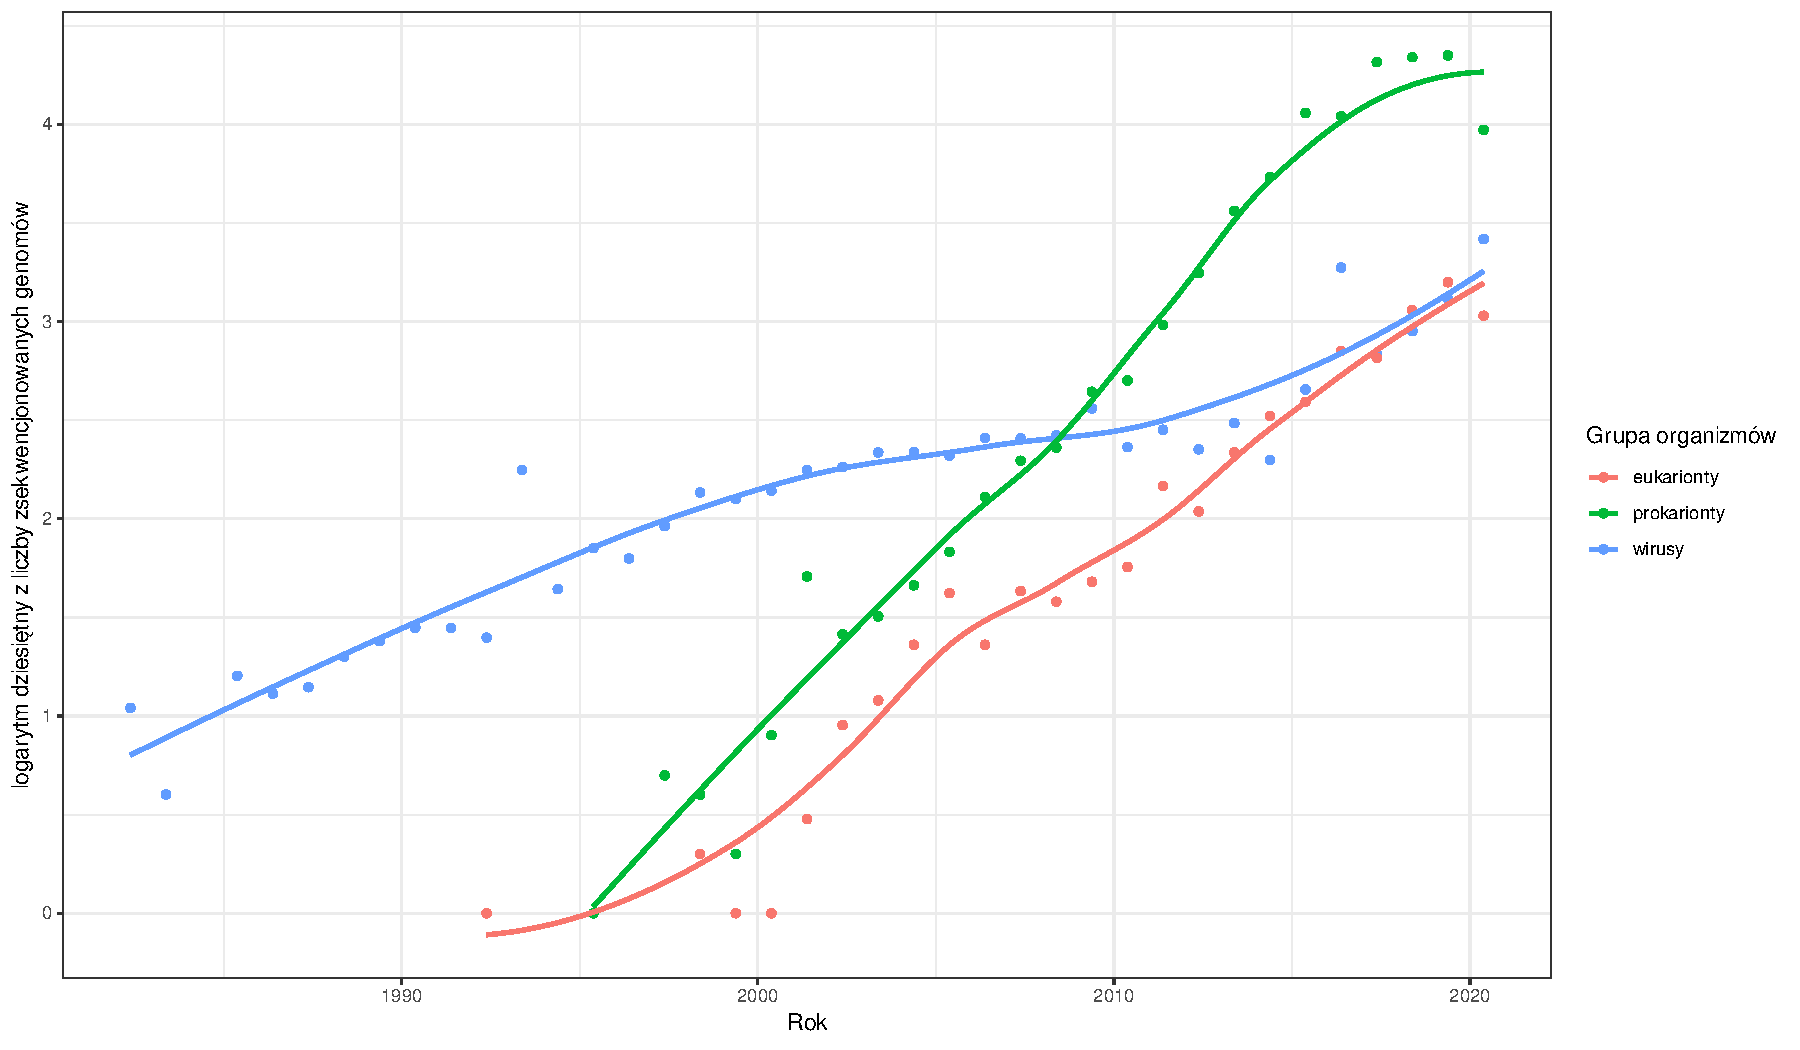
\includegraphics[width=\textwidth]{./sequenced_genomes.pdf}
	\caption{Ostatnie lata odnotowują bardzo szybki wzrost sekwencjonowanych genomów. Sekwencjonowanie genomów wirusowych odnotowuje jednak o wiele niższy wzrost niż prokariotycznych i eukariotycznych. Wykres przedstawia ilość genomów dodanych do bacy NCBI \autocite{NCBI} w danym roku.}\label{fig::seq_trends}

	\footnotetext{Autor pracy jest autorem wykresu, opracowanego na podstawie internetowej bazy danych NCBI. Kod wykresu można znaleźć pod adresem \textit{https://github.com/jakubguzek/metody-biol-mol}}
\end{tcolorbox}
\end{figure}

Jak wspomniano wyżej, dzisiejsze metody umożliwiają sekwencjonowanie całych genomów w stosunkowo niedługim czasie, a wraz z opracowywaniem metod sekwencjonowania trzeciej i czwartej generacji możliwe będzie sekwencjonowanie ich w czasie rzeczywistym \autocite{Brown2019}. Prócz tego mikromacierze, hybrydyzacja i chromatografia powinowactwa umożliwiają badanie transkryptów genów i tworzenie transkryptomów (zbiorów wszystkich cząsteczek RNA w komórce) oraz zestawu białek komórkowych zwanego proteomem. Daje to możliwości badania komórki i interakcji molekularnych jakie są w niej obecne i umożliwia rozwój takim dziedzinom jak biologia systemów i interaktomika. Temu wszystkiemu towarzyszy oczywiście doskonalenia narzędzi informatycznych używanych do badań z zakresu \textit{-omics}, którym zajmuje się bioinformatyka.

Które z tych metod są wykorzystywane w badaniu wirusów? Wiele z nich zostało opracowanych przy pracy na wirusach, zwłaszcza w początkowych dniach biologii molekularnej, gdy sekwencjonowanie genomów było przedsięwzięciem wielokrotnie trudniejszym niż dzisiaj, gdyż genomy wirusowe są niedużych rozmiarów, były więc atrakcyjnym materiałem badawczym. Wraz z postępem w tej dziedzinie wzrosła jednak ilość sekwencjonowanych genomów prokariotycznych i eukariotycznych (Rysunek \ref{fig::seq_trends}). Na dzień dzisiejszy w bazie danych NCBI jest ponad 30 tys. rekordów dla genomów wirusowych i ponad 200 tys. dla genomów prokariotycznych.

\section{Sekwencjonowanie genomu}

Celem badań genomicznych jest poznanie sekwencji genomu badanego organizmu lub wirusa, Techniki używane w czasie projektów poznawania genomów noszą nazwę sekwencjonowania i polegają zwykle na sekwencjonowaniu krótkich fragmentów wyizolowanych z badanych próbek. Długości takich sekwencji waha się w zależności od używanej metody od 750 bp. do 700 Mb., a w wypadku metod trzeciej i czwartej generacji wirtualnie nie ma ograniczenia gdyż zachodzi w czasie rzeczywistym \autocite{Brown2019}.

Pierwsze metody sekwencjonowania genomu zostały opracowane w latach 70 XXw. \textbf{Metoda terminacji łańcucha} opracowana przez F. Sangera \autocite{Sanger1977}, szybko zyskała popularność i mimo wielu ograniczeń jest stosowana do dzisiaj w projektach sekwencjonowania niedużych genomów \autocite{Brown2000} i mniejszych fragmentów. Drugą metodą opracowaną w tej samej dekadzie było \textbf{sekwencjonowanie metodą degradacji chemicznej}, które nie zyskało takiej popularności jak metoda terminacji łańcucha ze względu na wykorzystywanie toksycznych odczynników i mniejsze możliwości automatyzacji.

Techniki opracowane w kolejnych latach, umożliwiające sekwencjonowanie wielu tysięcy fragmentów jednocześnie nazywamy \textbf{technikami sekwencjonowania nowej generacji}.

\subsection{Sekwencjownoanie pierwszej generacji}

Jak już wspomniano metoda terminacji łańcucha opracowana przez F. Sangera, w latach 70, zyskała na popularności i została wdrożona w wielu dużych projektach takich jak Projekt Poznania Genomu Człowieka \autocite{IHGSC2001}. Oparta jest ona na zdolności jednoniciowego DNA, różniącego się długością do rozdziału na żelu poliakryloamidowym poprzez elektroforezę.

Elektroforezę taką można przeprowadzić w kapilarze o długości 50-80cm i średnicy $\sim 0,1mm$, co umożliwia rozdzielenie cząsteczek jednoniciowego DNA o długości do 1500 bp.

Samo sekwencjonowanie przeprowadza się przy użyciu polimerazy DNA, o pożądanych cechach takich jak:
\begin{itemize}
\item duża procesywność
\item nieznaczna aktywność egzonukleazy $5'\rightarrow3'$ lub jej brak
\item nieznaczna aktywność egzonukleazy $3'\rightarrow5'$ lub jej brak
\end{itemize}

W pierwszym etapie przyłączeniu do sekwencjonowanych fragmentów ulegają oligonukleotydy, pełniące rolę starterów dla syntezy nowej, komplementarnej nici DNA. W tej reakcji oprócz czterech, typowych trifosforanów deoksyrybonukleotydów (dATP. dCTP, dGTP, dTTP) jako substraty biorą udział także trifosforany dideoksyrybonukleotydów (ddATP, ddCTP, ddGTP, ddTTP), wyznakowane charakterystycznymi dla siebie znacznikami fluorescencyjnymi.

Polimeraza DNA przyłącza dideoksyrybonukleotydy tak samo jak przyłączyłaby normalne deoksyrybonukleotydy, jednak przyłączenie ddNTP uniemożliwia dalsze wydłużanie łańcucha i prowadzi do terminacji syntezy, na skutek braku grupy 3' hydroksylowej. ddNTPs są w środowisku reakcji obecne w stężeniu niższym niż dNTPs, terminacja nici zachodzi więc w różnych odległościach od startera, powodując powstanie wielu nici o różnych długościach, z których każda ma na końcu terminalnym dideoksyrybonukleotyd.

\begin{figure}[h]
\begin{tcolorbox}
	\centering
	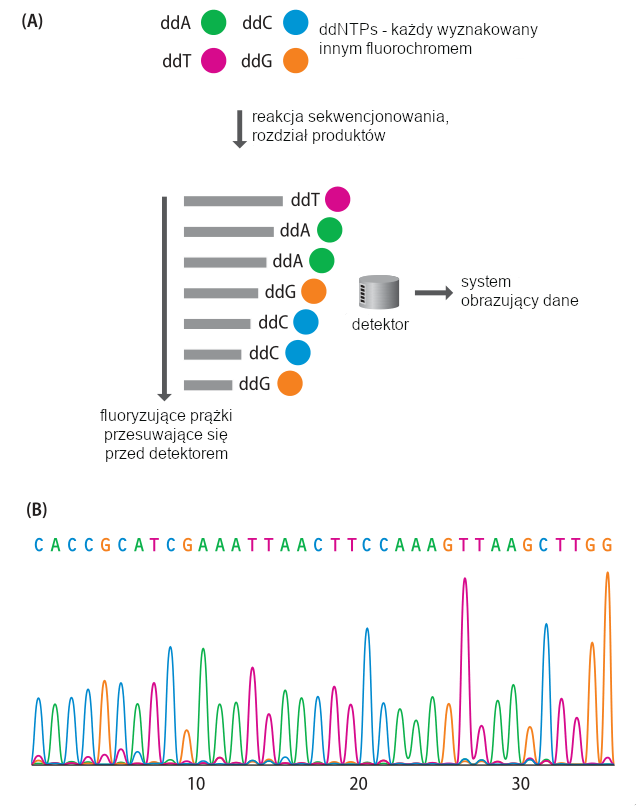
\includegraphics[width=\textwidth]{./figury/sekwencja_metoda_terminacji.png}
	\caption{Odczytywanie sekwencji uzyskanej podczas sekwencjonowania metodą terminacji łańcucha (A) Każdy dideoksyrybonukleotyd jest wyznakowany innym fluorochromem. Detektor fluorescencji wykrywa jaki ddNTP znajduje się w przesuwającym się przed nim prążku i przesyła informacje do systemu obrazującego przetworzone dane. (B) Wydruk sekwencjonowania DNA (Na podstawie Brown 2019)}\label{fig::seq_chain_term}
\end{tcolorbox}
\end{figure}

Aby ustalić sekwencje badanego fragmentu należy rozdzielić uzyskane w tej procedurze fragmenty na żelu poliakryloamidowym i ustalić która cząsteczka kończy się jakim ddNTP (Rysunek \ref{fig::seq_chain_term}). Robi się to przy pomocy detektora fluorescencji, który rozróżnia znaczniki dołączone do poszczególnych dideoksyrybonukleotydów.

Zastosowanie techniki terminacji łańcucha umożliwia sekwencjonowanie fragmentów o długości do 750 bp. Automatyczne sekwenatory z licznymi kapilarami mogą jednak sekwencjonować wiele fragmentów równolegle co znacznie zwiększa możliwości tej metody \autocite{Brown2019}

Pierwszymi zsekwencjonowanymi genomami były genomy Bakteriofaga MS2 (ssRNA) i Bakteriofaga $\Phi X174$ \autocite{Sanger1978} (DNA), czyli genomy wirusowe. Genomy wirusów są relatywnie łatwe do zsekwencjonowania ze względu na ich (zwykle) nieduże rozmiary. Genom Bakteriofaga $\Phi X714$ został zsekwencjonowany metodą terminacji łańcucha.

\subsection{Sekwencjonowanie nowej generacji}

Metody nowej generacji pozwalają uzyskać dużą ilość danych, w krótkim czasie dzięki czemu umożliwiają złożenie nawet dużych genomów w znacznie krótszym czasie niż metoda terminacji łańcucha. Niosą one za sobą zwykle wyższe wymagania obliczeniowe, jednak w dzisiejszych czasach nie jest to dużym problemem, gdyż moc obliczeniowa konieczna do analizy tych danych jest względnie tania.

Istnieje wiele metod nowej generacji jednak ich wspólną cechą jest etap poprzedzający właściwe sekwencjonowanie, polegający na przygotowaniu biblioteki fragmentów DNA. Konstruowanie takiej biblioteki polega na unieruchamianiu fragmentów na podłożu stałym w formacie macierzy masowo równoległej. Umożliwia to przeprowadzenie wielu reakcji sekwencjonowania jednocześnie. Fragmenty na takiej macierzy mają zwykle niewielką długość (do 500 bp.). Unieruchamianie fragmentów przeprowadza się zwykle jednym z dwóch sposobów:
\begin{itemize}
	\item Ligacja końców fragmentów z adaptorami, czyli krótkimi dwuniciowymi kawałkami DNA, których sekwencje są komplementarne do oligonukleotywów związanych z mikromacierzą.
	\item Wykorzystanie podłoża w postaci małych metalicznych kulek pokrytych białkiem streptawidyną. W tym wypadku fragmenty DNA ligowane są z adaptorami, które mają przyłączone na końcach 5' znaczniki w postaci biotyny, która może tworzyć silne wiązania ze streptowidyną.
\end{itemize}
\begin{figure*}[btp]
	\begin{tcolorbox}
		\centering
		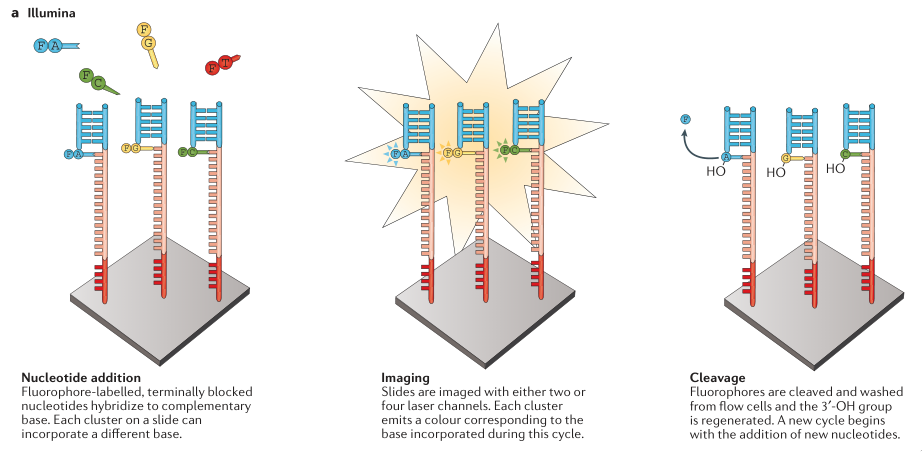
\includegraphics[width=\textwidth]{./figury/illumina.png}
		\caption{\textbf{Sekwencjonowanie metodą cyklicznej odwracalnej terminacji}. Po amplifikacji fragmentów na macierzy, mieszanina starterów, i zmodyfikowanych nukleotydów jest dodana na macierz, wraz z polimerazą DNA. Każdy nukleotyd ma grupę blokującą przy 3' węglu deoksyrybozy (tutaj grupa 3'-O-metyloazydkowa) i jest oznaczony charakterystycznym dla siebie fluorochromem (F),  W czasie każdego cyklu fragmenty ulegną wydłużeniu o jeden nukleotyd. Wówczas detektor mierzy fluorescencję z każdego miejsca na macierzy, Na koniec fluorochrom i grupa blokująca są wycinane \autocite{Godwin2016}.}\label{fig::illumina}
	\end{tcolorbox}
\end{figure*}
Następnie unieruchomione fragmenty amplifikuje się wykorzystując PCR, co umożliwia wytworzenie wystarczającej ilości kopii do zsekwencjonowania \autocite{Godwin2016}\autocite{Brown2019}.

Dalsze kroki różnią się znacząco w różnych metodach.

\textbf{Sekwencjonowanie metodą odwracalnej terminacji}, nazywana też sekwencjonowaniem w technologii Illumina (Rysunek \ref{fig::illumina}) wykorzystuje zmodyfikowane nukleotydy, które po dołączeniu przez polimerazę wydłużanego łańcucha powodują terminację. Metoda ta tym różni się jednak od metody F. Sangera, że tutaj terminacja jest odwracalna. Zaraz po odczytaniu na jakim nukleotydzie nastąpiła terminacja można z niego usunąć grupę blokującą, dołączoną do węgla 3' deoksyrybozy. Grupą blokującą może być znacznik fluorescencyjny, charakterystyczny dla danego nukleotydu. Mieszanina reakcyjna zawiera w wybranym momencie tylko zmodyfikowane nukleotydy, każdy krok syntezy powoduje więc terminację łańcucha. W każdym kroku detektor wykrywa znacznik fluorescencyjny i identyfikuje terminalny nukleotyd, Grupa blokująca jest następnie usuwana enzymatycznie. Metoda ta generuje odczyty o długości sekwencji do 300 bp. jednak dzięki wykorzystaniu macierzy masowo równoległej można uzyskać sekwencje o łącznej długości $20\,000$ Mb. \autocite{Godwin2016}.

\textbf{Sekwencjonowanie 454}, zwane także pirosekwencjonowaniem polega na wykrywaniu błysków chemoiluminescencji, wytwarzanych przez adenylilotransferazę siarczanową, rozkładającą cząsteczki pirofosforanu ($\mathrm{PP_{i}}$), który uwalniany jest przy każdym dołączeniu dNTP do syntezowanej nici. Każdy deoksyrybonukleotyd jest dodawany oddzielnie, jeden po drugim, a wzór chemoiluminescjencji jest wykorzystywany do ustalenia kolejności dodawania nukleotydów do nici przez polimerazę DNA \autocite{Brown2019} \autocite{Godwin2016}.

\textbf{Sekwencjonowanie ion torrent} wykorzystuje podobne podejście do sekwencjonowanie 454, system detekcji wykrywa jednak jony wodorowe, które są uwalniane wraz z $\mathrm{PP_{I}}$, zamiast samego pirofosforanu. Uwalnianie jony są wykrywane przez wrażliwy na jony tranzystor polowy (\textbf{ISFET} -- \textit{ion-sensitive field effect transistor}) \autocite{Brown2019}.

\textbf{Sekwencjonowanie przez ligację i wykrywanie oligonukleotydów} (\textbf{SOLiD} -- \textit{sequencing by oligonucleotide ligations and detection}). Metoda ta korzysta z innego podejścia niż metody nowej generacji opisane do tej pory. Sekwencja generowana jest na podstawie sygnałów hybrydyzacji zbioru oligonukleotydów, komplementarnych do sekwencji sekwencjonowanego fragmentu matrycowego. Cały proces rozpoczyna przyłączenie primera do sekwencji końcowych adaptorów na matrycy. Później dodawana jest mieszanina 1024 5-nukleotydowych oligonukleotydów\footnote{reprezentują one każdą możliwą kombinację 5 nukleotydów} wraz z enzymem ligazą (Rysunek \ref{fig::solid}). Sekwencja jednego z tych oligonukleotydów musi być komplementarna z odcinkiem matrycy bezpośrednio sąsiadującym ze starterem -- taki oligonukleotyd hybrydyzuje z matrycą w tym miejscu i ulega ligacji do primera. Kolejny oligonukleotyd, komplementarny do sekwencji fragmentu matrycy za tym poprzednio dołączonym, ulega hybrydyzacji i ligacji do poprzedniego. Powtarza się to aż do całkowitego pokrycia badanego fragmentu. Każdy taki 5-nukleotydowy fragment jest wyznakowany fluorochromem, przy czym wykorzystane są ogólnie tylko cztery fluorochromy. Z uwagai na rodzaj znacznika fluorescencyjnego oligonukleotydy podzielone są na 4 rodziny, a których każda zawiera po 256 sekwencji -- o przynależności do danej rodziny decyduje kombinacja pierwszych dwóch nukleotydów we fragmencie. Wykrycie znacznika związanego z hybrydyzującym oligonukleotydem pozwala więc przypisać dwa nukleotydy w 5-nukleotydowej sekwencji. Daje to niepełną i niejednoznaczną sekwencję, dlatego proces sekwencjonowania powtarzany jest z wykorzystaniem drugiego primera, przyłączającego się w pozycji przesuniętej o jeden nukleotyd względem poprzedniego startera -- powtarza się to aż każdy nukleotyd w sekwencji jest odczytany dwukrotnie. W sekwencjonowaniu SOLiD otrzymuje się krótsze odczyty niż w pozostałych metodach nowej generacji (od 50 do 75 bp.), ale są to odczyty wyjątkowo dokładne. Dodatkowo z uwagi na sposób w jaki zbierane są dane oraz jaka jest ich struktura technika ta jest wymagająca obliczeniowe, co jednak -- jak już wcześniej wspomniano, nie jest w dzisiejszych czasach dużą wadą ze względu na stosunkowo tanie zasoby komputerowe. \autocite{Godwin2016} \autocite{Brown2019}

\begin{figure*}[btp]
	\begin{tcolorbox}
		\centering
		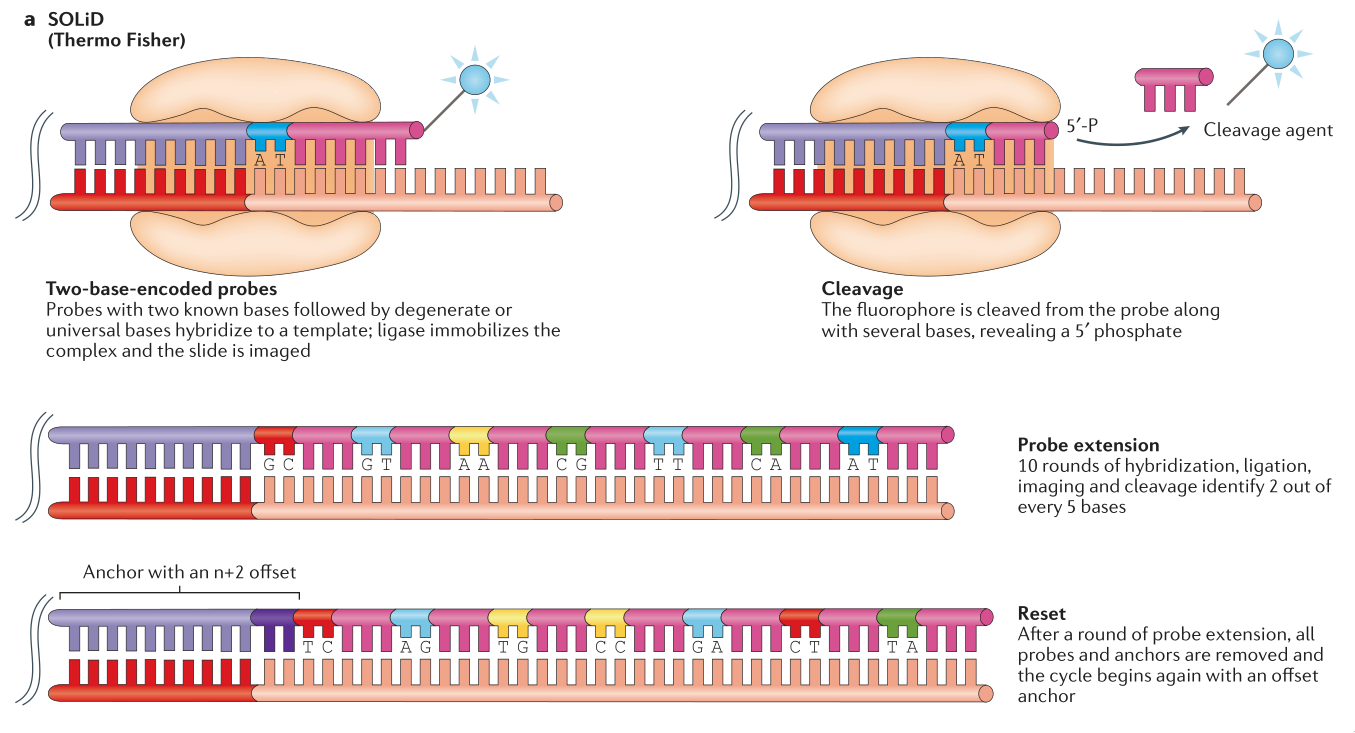
\includegraphics[width=\textwidth]{./figury/solid.png}
		\caption{\textbf{Sekwencjonowanie przy użyciu ligacji}. Sekwencjonowanie metodą SOLiD. Po skonstruowaniu biblioteki fragmenty są sekwencjonowane przez ligację. Więcej informacji w tekście (Na podstawie Godwin 2016)}\label{fig::solid}
	\end{tcolorbox}
\end{figure*}

\subsection{Sekwencjonowanie trzeciej i czwartej\\ generacji}

Ograniczeniem metod nowej generacji jest konieczność chwilowego wstrzymania elongacji łańcucha w celu przeprowadzenia pomiaru, co znacznie spowalnia proces sekwencjonowania. Metody umożliwiające odczytywanie sekwencji w tempie działania polimerazy bez konieczności zatrzymywania reakcji nazywane są metodami trzeciej generacji, lub sekwencjonowaniem w czasie rzeczywistym.

\textbf{Single-molecule realtime sequencing}, polega na śledzeniu kopiowaniu pojedynczej matrycy DNA przy pomocy systemu optycznego nazwanego \textit{zero-mode waveguide}. Substratami reakcji są tutaj wyznakowane fluorescencyjnie dNTPs. Wspomniany system optyczny jest precyzyjny iż nie ma konieczności zatrzymywania reakcji na żadnym etapie elongacji łańcucha.  Znacznik fluorescencyjny jest usuwany zaraz po dołączeniu nukleotydu. Metoda ta umożliwia wykonywanie odczytów o długości do $20\,000$ bp. \autocite{Brown2019}.

\textbf{Sekwencjonowanie w nanoporach} umożliwia odczytanie sekwencji fragmentu DNA, bez konieczności jego kopiowania i zwane jest metodą czwartej generacji. Wykorzystuje membranę z porami, o średnicy wystarczającej do przejścia przez nie cząsteczki DNA \autocite{Feng2015}. Przez membranę przepuszczany jest prąd elektryczny, co powoduje jej polaryzację. Wprowadzona do nanoporu cząsteczka jest dwuniciowa, ale ulega rozpleceniu przy użyciu zasocjowanej do poru helikazy. Finalnie przez nanopor przechodzi jedna nić DNA, która przechodząc zaburza prąd przepływu jonów przez por. Umożliwia to wykrycie, jaki nukleotyd przechodzi w dowolnym momencie, gdyż na skutek różnicy w strukturze poszczególnych nukleotydów prąd jonowy jest zaburzany w różny sposób. \autocite{Brown2019}

\begin{figure}[bt]
\begin{tcolorbox}
	\centering
	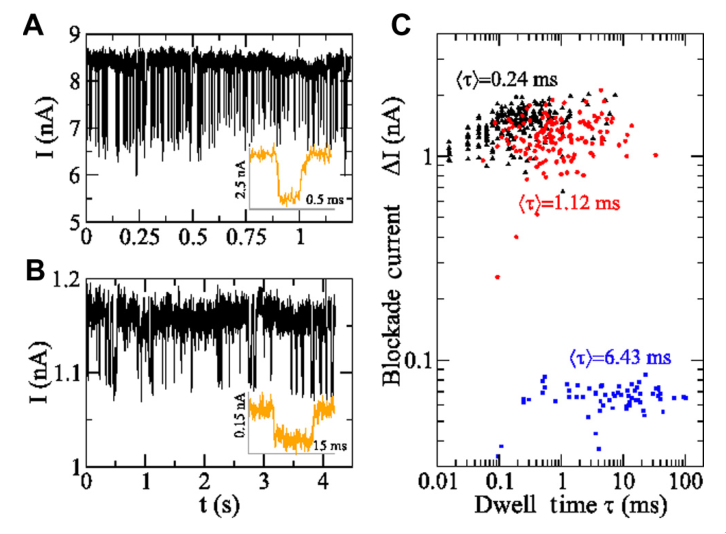
\includegraphics[width=\textwidth]{./figury/nanopore_experimental.png}
	\caption{Eksperymentalne wyniki przemieszczania ssDNA przez nanopor o średnicy 9nm}
\end{tcolorbox}
\end{figure}

\section{Anotacja genomu i badanie transkryptomu}

 Mogłoby się wydawać, że z punktu widzenia wirusologii badanie transkryptomu nie jest bardzo istotne -- genomy RNA wirusów w ogóle nie podlegają transkrypcji, a wszystkie wirusy są pasożytami aparatu translacyjnego a nie transkrypcyjnego. Jednak struktura genomowego RNA wirusów RNA jest bardzo podobna do struktury komórkowych RNA, przy czym genomowy RNA wirusów jest niejednokrotnie bardziej skomplikowany niż RNA organizmów komórkowych. Wirusy muszą sprostać wyzwaniu zawarcia jak największej ilości informacji w jak najmniejszej ilości kwasu nukleinowego, stad dużo informacji przenosi u niech nie tylko sama sekwencja nukleotydów w kwasie nukleinowym co trójwymiarowy kształt cząsteczki tego kwasu. Wiele miejsc jest wskutek wyrafinowanego pozwijania wirusowych genomów RNA niedostępnych sterycznie dla białek, a inne miejsca muszą przyłączać się do rybosomów gospodarza łatwiej niż transkrypty komórkowe, aby umożliwić efektywną ekspresję genów wirusa.. Metody transkryptomiczne pełnią istotną rolę w ustaleniu sekwencji genomów RNA wirusów, z której nie tylko można wnioskować o kodowanych przez ten genom białkach, ale także o niuansach wpływu kształtu genomu na jego zachowanie w patogenezie danego wirusa \autocite{Piekarowicz2013}. Stąd metody takie jak RT-PCR (\textit{reverse transcription PCR}), tworzenie klonów zawierających cDNA, i tradycyjne sekwencjonowanie znajdują zastosowanie w badaniach wirusologicznych. Metody anotacji genomu umożliwiają przypisanie roli poszczególnym fragmentom wirusowych genomów.

Również nowoczesne metody transkryptomiczne takie jak RNA-Seq i RACE są stosowane przy badaniu wirusów -- na przykład przy badaniu funkcji poszczególnych elementów wirusowego genomu lub identyfikacji promotorów \autocite{Steger2001}

\subsection{RNA-Seq}

RNA-Seq jest to zastosowanie technologii Illuminy lub innej metody sekwencjonowania wysokoprzepustwoego do biblioteki przygotowanej z cDNA, a nie DNA. Odczyty sekwencji odpowiadają segmentom transkryptów oryginalnej cząsteczki RNA. Odczyty takie można zmapować na genomie referencyjnym. Analiza taka jest problematyczna ze względu na to iż u organizmów eukariotycznych RNA ulega składaniu po transkrypcji. Prócz tego obróbka danych uzyskanych tą metodą jest skomplikowana pod kątem obliczeniowym \autocite{Brown2019}

\subsection{RT-PCR i RACE}

Klasyczne metody hybrydyzacji nie dają informacji na temat położenia genów kodujących transkrypt w genomie. RT-PCR wykorzystuje jako matrycę jednoniciowy RNA, na którego matrycy syntezowana jest nić cDNA, która następnie podlega amplifikacji, w sposób typowy dla normalnej metody PCR.

Szczególną wersją RT-PCR jest RACE \textit{rapid amplification of cDNA ends}). W najprostszej formie tej metody jeden primer jest specyficzny dla początku danego genu i wiąże się z mRNA będącym transkryptem tego genu. Następuje synteza cDNA na matrycy mRNA. Jako że kopiowaniu ulega tylko fragment mRNA to synteza konczy się przedwcześnie i jeden koniec powstałego cDNA dokładnie odpowiada początkowi matrycy mRNA. Do końca 3' cDNA transferaza terminalna dodaje nukleotydy adeninowe, tworząc ogon poli(A). Kolejny primer wiąże się z sekwencją poli(A) w pierwszym cyklu PCR i prowadzi do amplifikacji powstałej cząsteczki, której sekwencja pokazuje początek transkryptu. \autocite{Brown2019}.

\section{Badanie proteomu}

Szczególnie ważne w badaniu funkcjonowania wirusów jest badania funkcji wytwarzanych przez nie białek i interakcji między nimi. Wirusy nie posiadają skomplikowanego metabolizmu jak komórki. Nie są w stanie wytwarzać energii, nie mają własnego układu enzymatycznego ani translacyjnego i to właśnie czyni jest obligatoryjnymi pasożytami.

Genom wirusa niezależnie czy DNA czy RNA nie koduje zazwyczaj dużej ilości białek (rzecz jasna istnieją wyjątki -- genomy niektórych wirusów potrafią być większe niż genomy bakteryjne). Białka, które są kodowane przez genom większości wirusów można podzielić na strukturalne i niestrukturalne. Wśród białek strukturalnych można wyróżnić m. in. białka kapsydu i białka macierzy, a niestrukturalnych enzymy proteolityczne (często odpowiedzialne za cięcie wirusowych poliprotein), lub regulatory tranlacjim czy replikacji genomu wirusa \autocite{Piekarowicz2013}.

Metody proteomiczne takie jak krystalografia i  Cryo-EM umożliwiają nie tylko szczegółowe poznanie struktury białek, ale także badanie interakcji między nimi. Jest to szczególnie istotne dla badań wirusologicznych dotyczących składania wirionów oraz ich wnikania do komórek \autocite{Rossmann2000}.

\subsection{Cryo-electron microscopy}

Mikroskopia krioelektronowa jest metodą umożliwiającą otrzymanie bardzo dokładnego obrazu struktury przestrzennej białek, bez konieczności hodowania kryształu, co jest jednym z głównych ograniczeń krystalografii rentegnowskiej, która jest klasyczną i jedną z najpopularniejszych metod badania struktury białek.

Pierwszym etapem w tej metodzie jest otrzymanie ultraczystego roztworu badanego białka, który następnie rozprowadza się na cienkiej specjalnie spreparowanej siatce. Warstwa roztworu musi być możliwie najbardziej cienka, tak aby wszystkie cząsteczki białka znajdujące się w roztworze znajdowały się w jednej płaszczyźnie i nie nachodziły na siebie. Taki preparat następnie poddaje się gwałtownemu mrożeniu w ciekłym metanie, aby otrzymać badany roztwór w postaci anizotropowego, bezpostaciowego ciała stałego. Otrzymany w ten sposób cienki skrawek poddaje się obserwacji pod mikroskopem elektronowym (również w możliwie najniższej temperaturze). Wykonuje się zdjęcia mikroskopowe cząsteczek białka -- naturalnie cząsteczki zostają zamrożone w różnych pozycjach, co umożliwia otrzymanie wielu zdjęć cząsteczki z różnych perspektyw. \autocite{Baldwin1988}. Takie dane można podać analizie komputerowej i otrzymać model białka o wysokiej rozdzielczości sięgającej nawet 1\r{A}.

Metoda ta umożliwia nawet otrzymywanie trójwymiarowej struktury całych wirionów \autocite{Adrian1984}.

\section{Podsumowanie}

Wymienione metody są tylko jednymi z wielu metod biologii molekularnej stosowanych na całym świecie w badaniach wirusologicznych i nie tylko. Nie omówiono tutaj szczegółowo elementarnych metod biologii molekularnej takich jak PCT, tworzenie bibliotek klonów, etc. a w zamian za to skupiono się na metodach nowocześniejszych i mniej elementarnych. Wybór ten jest rzecz jasna nader arbitralny i odzwierciedla raczej luźne powiązanie wewnętrzne. Niektóre z tych technik są szerzej stosowane w wirusologii niż inne. Niektóre metody wywodzą się od eksperymentów na wirusach, a inne są do takiej pracy wtórnie dostosowane.

W pracy tej nie zagłębiano się szczegółowo w analizę danych produkowanych przez poszczególne metody. Jest to rzecz jasna niezwykle istotny etap we wszystkich badaniach, zwłaszcza w dzisiejszych czasach. Niejednokrotnie skrupulatna analiza danych jest ważniejsza niż sama metoda jaką je otrzymano. Jest to pole należące głównie do bioinformatyki i odnotowuje niezwykle szybki rozwój, z algorytmami opartymi na big data i uczeniu maszynowym na czele.

To jak ważne są badania wirusologiczne jest szczególnie widoczne w obecnym czasie, gdy świat mierzy się z pandemią SARS-CoV-2. Badania dotyczące tego wirusa są zdominowane przez techniki biologii molekularnej i ,\textit{-omiczne}, co bezpośrednio wskazuje na ich istotność.

\printbibliography

\end{document}
